%
% $Id: slides.tex 4228 2006-06-21 21:55:12Z jjamor $
%
%
% Compilar a .pdf con LaTeX (pdflatex)
% Es necesario instalar Beamer (paquete latex-beamer en Debian)
%

%
% Gráficos:
% Los gráficos pueden suministrarse en PNG, JPG, TIF, PDF, MPS
% Los EPS deben convertirse a PDF (usar epstopdf)
%

\documentclass{beamer}
\usetheme{Warsaw}
\usebackgroundtemplate{
\includegraphics[width=\paperwidth]{format/libresoft-bg.png}}
\usepackage[spanish]{babel}
\usepackage[utf8]{inputenc}
\usepackage{graphics}
\usepackage{amssymb} % Simbolos matematicos

%\definecolor{libresoftgreen}{RGB}{162,190,43}
%\definecolor{libresoftblue}{RGB}{0,98,143}

%\setbeamercolor{titlelike}{bg=libresoftgreen}

%% Metadatos del PDF.
\hypersetup{
  pdftitle={Free Software Developers},
  pdfauthor={José Gato, Teo Romera},
  pdfcreator={GSyC/Libresoft},
  pdfproducer=PDFLaTeX,
  pdfsubject={Free Software Engineering},
}
%%

\begin{document}

\title{Free Software Developers}
\subtitle{Master on Free Software}
\institute{\{jgato,teo\}@gsyc.es\\
GSyC/LibreSoft}
\author{José Gato, Teo Romera}
\date{28-29 November 2008}

\frame{
\maketitle
\begin{center}

\includegraphics[width=6cm]{format/gsyc-urjc}
\end{center}
}


% Si el titulo o el autor se quieren acortar para los pies de página
% se pueden redefinir aquí:
%\title{Titulo corto}
%\author{Autores abreviado}


%% LICENCIA DE REDISTRIBUCION DE LAS TRANSPAS
\frame{
~
\vspace{4cm}

\begin{flushright}
{\tiny
(cc) 2008-2010 José Gato, Teo Romera\\
(cc) 2007 Juanjo Amor, Gregorio Robles \\
  Some rights reserved. This work licensed under Creative Commons
  Attribution-ShareAlike License. To view a copy of full license, see
  http://creativecommons.org/licenses/by-sa/2.0/ or write to
  Creative Commons, 559 Nathan Abbott Way, Stanford,
  California 94305, USA.
%  Este documento (o uno muy similar) está disponible en \\
%  \url{http://gsyc.escet.urjc.es/~jjamor/}
}
\end{flushright}
}
%%


\section{Introduction}

\begin{frame}
\frametitle{FLOSS developers are nerds!}

\begin{center}

\includegraphics[width=8cm]{figs/nerd.jpg} \\
(Photo: Nerd, by The Infamous Gdub\\
\url{http://flickr.com/photos/theinfamousgdub/1765952198/})
\end{center}

\end{frame}

\begin{frame}
\frametitle{FLOSS developers are gods!}

\begin{center}
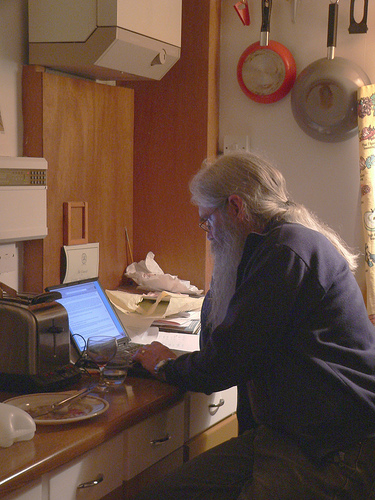
\includegraphics[width=4cm]{figs/hacker.jpg} \\
(Photo: Nerd, or perhaps hacker or geek?, by florriebassingbourn\\
\url{http://flickr.com/photos/75166820@N00/145258818/})
\end{center}

\end{frame}

\begin{frame}
\frametitle{Who are the Free Software Developers?}

\begin{itemize}
\item The open development model allow a large amount of work done by volunteer
developers
\item The possibility of having micro-contributions makes it difficult to know
more about developers
\item The distributed nature of the developer population makes it difficult to
know more about developers
\item Hence, there has been a lack of knowledge about the developers until
recently
\end{itemize}

\end{frame}


\begin{frame}
\frametitle{Who are the Free Software Developers?}

Questions to be answered:

\begin{itemize}
\item Who are the Free Software Developers? (gender, age, cultural level...)
\item Why do they develop Free Software?
\item Do they earn money when developing?
\item Where do they come from?
\end{itemize}

There have been many surveys since 2001 on this issue: WIDI (2001), FLOSS
(2002), FLOSS-US (2003), BCG Hacker Survey (2003), etc.

\end{frame}


\section{Personal Features}

\begin{frame}
\frametitle{Gender}

\begin{itemize}
\item 98\% male
\item 2\% female
\item (The statistical error lies around 3.5\%)
\item Does any discrimination exist? (see Krieger et al.)
\end{itemize}

\end{frame}

\begin{frame}
\frametitle{Age of Free Software Developers}

\begin{center}
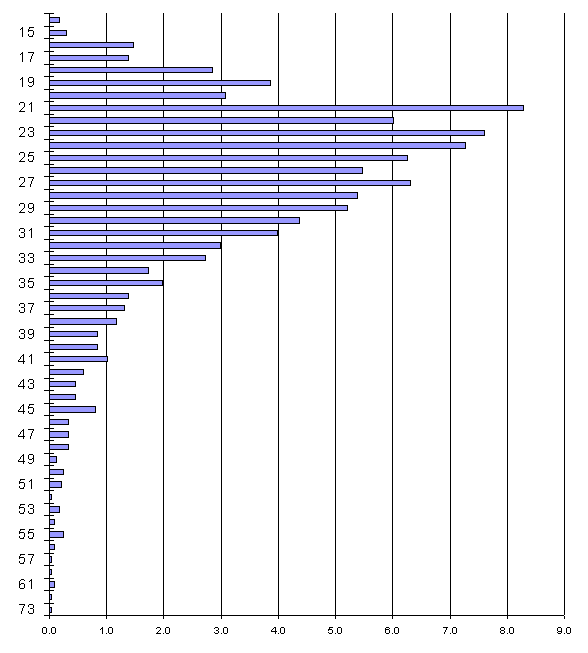
\includegraphics[width=6cm]{figs/age.png}
\end{center}

\end{frame}


\begin{frame}
\frametitle{Starting Age of Free Software Developers}

\begin{center}
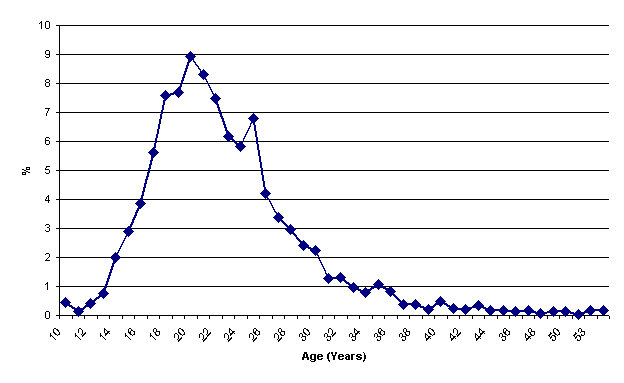
\includegraphics[width=8cm]{figs/starting-age.png}
\end{center}

\end{frame}


\begin{frame}
\frametitle{Educational Background of Free Software Developers}

\begin{center}
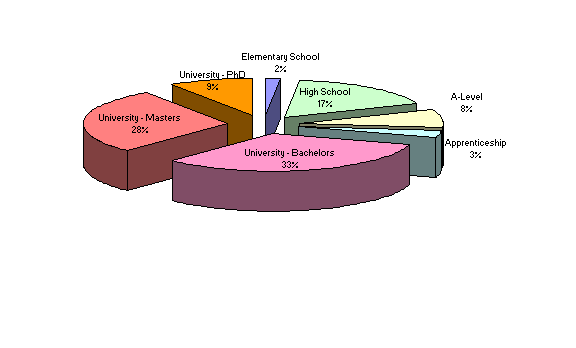
\includegraphics[width=10cm]{figs/educational-background.png}
\end{center}

\end{frame}


\begin{frame}
\frametitle{Professional Background of Free Software Developers}

\begin{center}
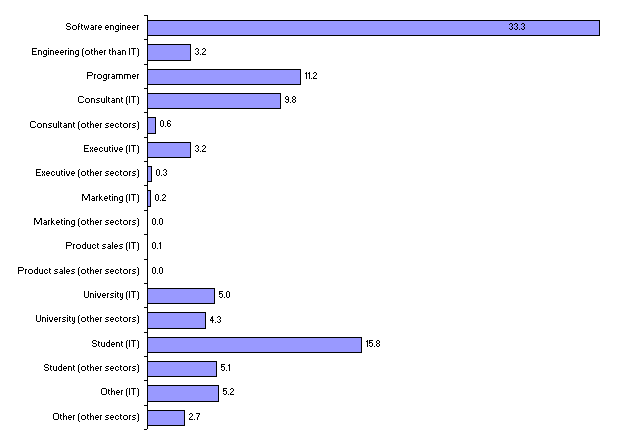
\includegraphics[width=8cm]{figs/professional-background.png}
\end{center}

\end{frame}


\section{Contribution attributes}

\begin{frame}
\frametitle{Time devoted to libre software projects}

\begin{center}
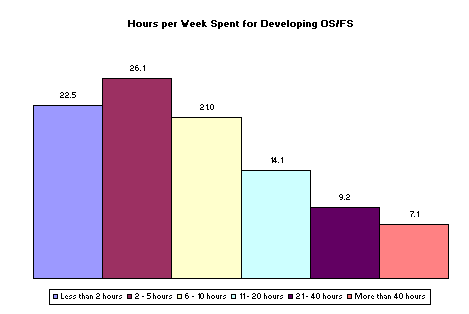
\includegraphics[width=8cm]{figs/hours-week.png}
\end{center}

\end{frame}

\begin{frame}
\frametitle{Time devoted to libre software projects compared to Proprietary Software}

\begin{center}
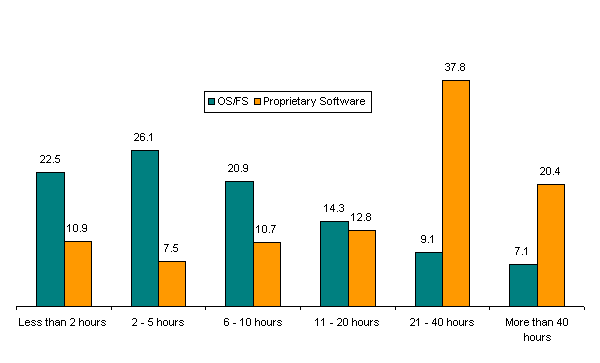
\includegraphics[width=8cm]{figs/TimeOSvsPS.png}
\end{center}

\end{frame}


\begin{frame}
\frametitle{Leadership and reputation}

\begin{center}
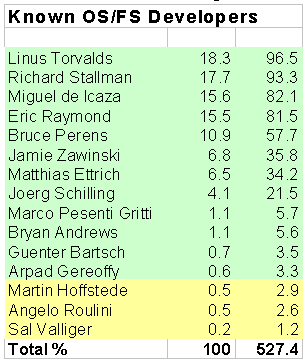
\includegraphics[width=6cm]{figs/leadership.png}
\end{center}

\end{frame}


\begin{frame}
\frametitle{Why Developers Join and Stay developing FLOSS}

\begin{center}
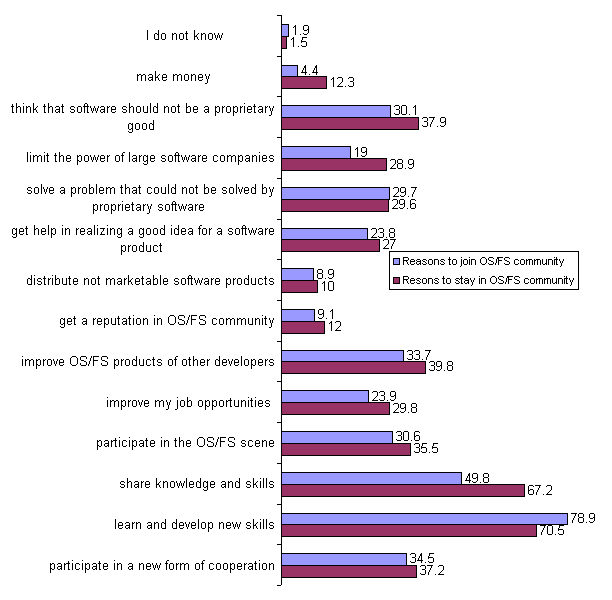
\includegraphics[width=7cm]{figs/why.png}
\end{center}

\end{frame}

\begin{frame}
\frametitle{Monetary rewards from developing FLOSS}

\begin{center}
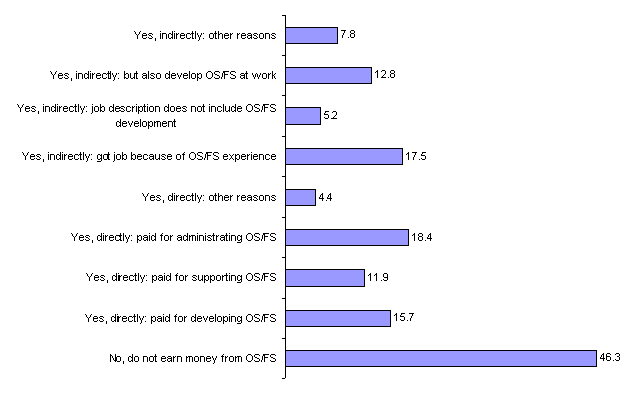
\includegraphics[width=9cm]{figs/money.png}
\end{center}

\end{frame}


\begin{frame}
\frametitle{Alignement Free Software vs. Open Source}

\begin{center}
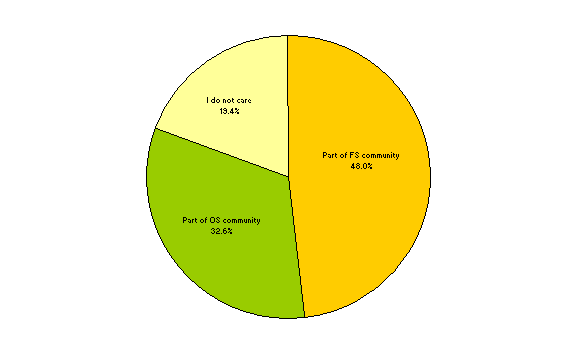
\includegraphics[width=9cm]{figs/FSvsOS.png}
\end{center}

\end{frame}


\begin{frame}
\frametitle{Alignement Free Software vs. Open Source}

\begin{center}
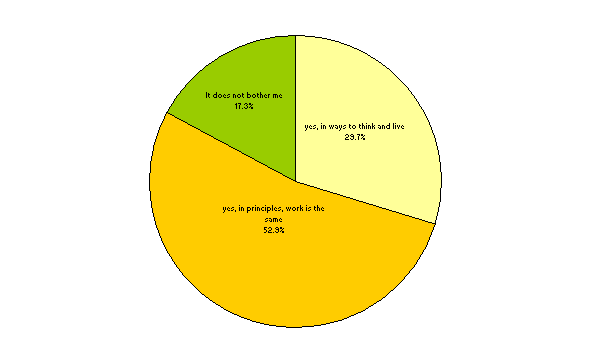
\includegraphics[width=9cm]{figs/FSvsOS2.png}
\end{center}

\end{frame}


\section{Geographic Origin}

\begin{frame}
\frametitle{Geographic Origin of FLOSS developers}

\begin{center}
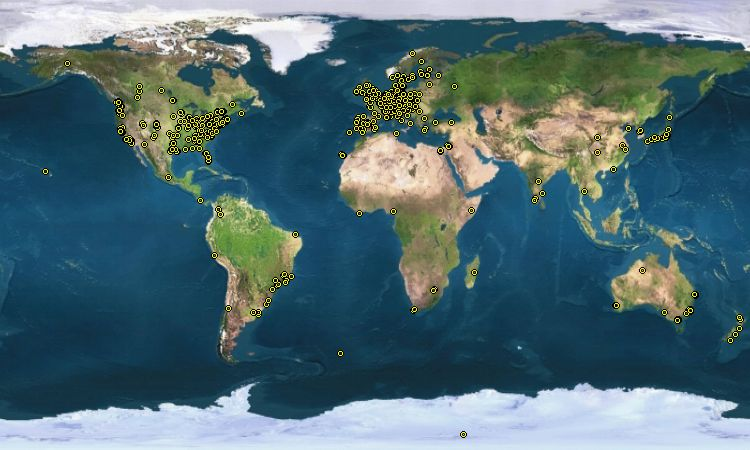
\includegraphics[width=11cm]{figs/developers-map.jpg}
\end{center}

\end{frame}

\begin{frame}
\frametitle{Conclusions}

The average developer

\begin{itemize}
\item Young male with a university degree
\item Tight link of the university with FLOSS
\item Pareto's Law in dedication hours
\item Non-monetary, non-egocentric motivations
\item Main motivation: sharing and learning
\item Good coding does not always mean reputation
\end{itemize}
\end{frame}

\begin{frame}
\frametitle{They are just normal people}

\begin{center}
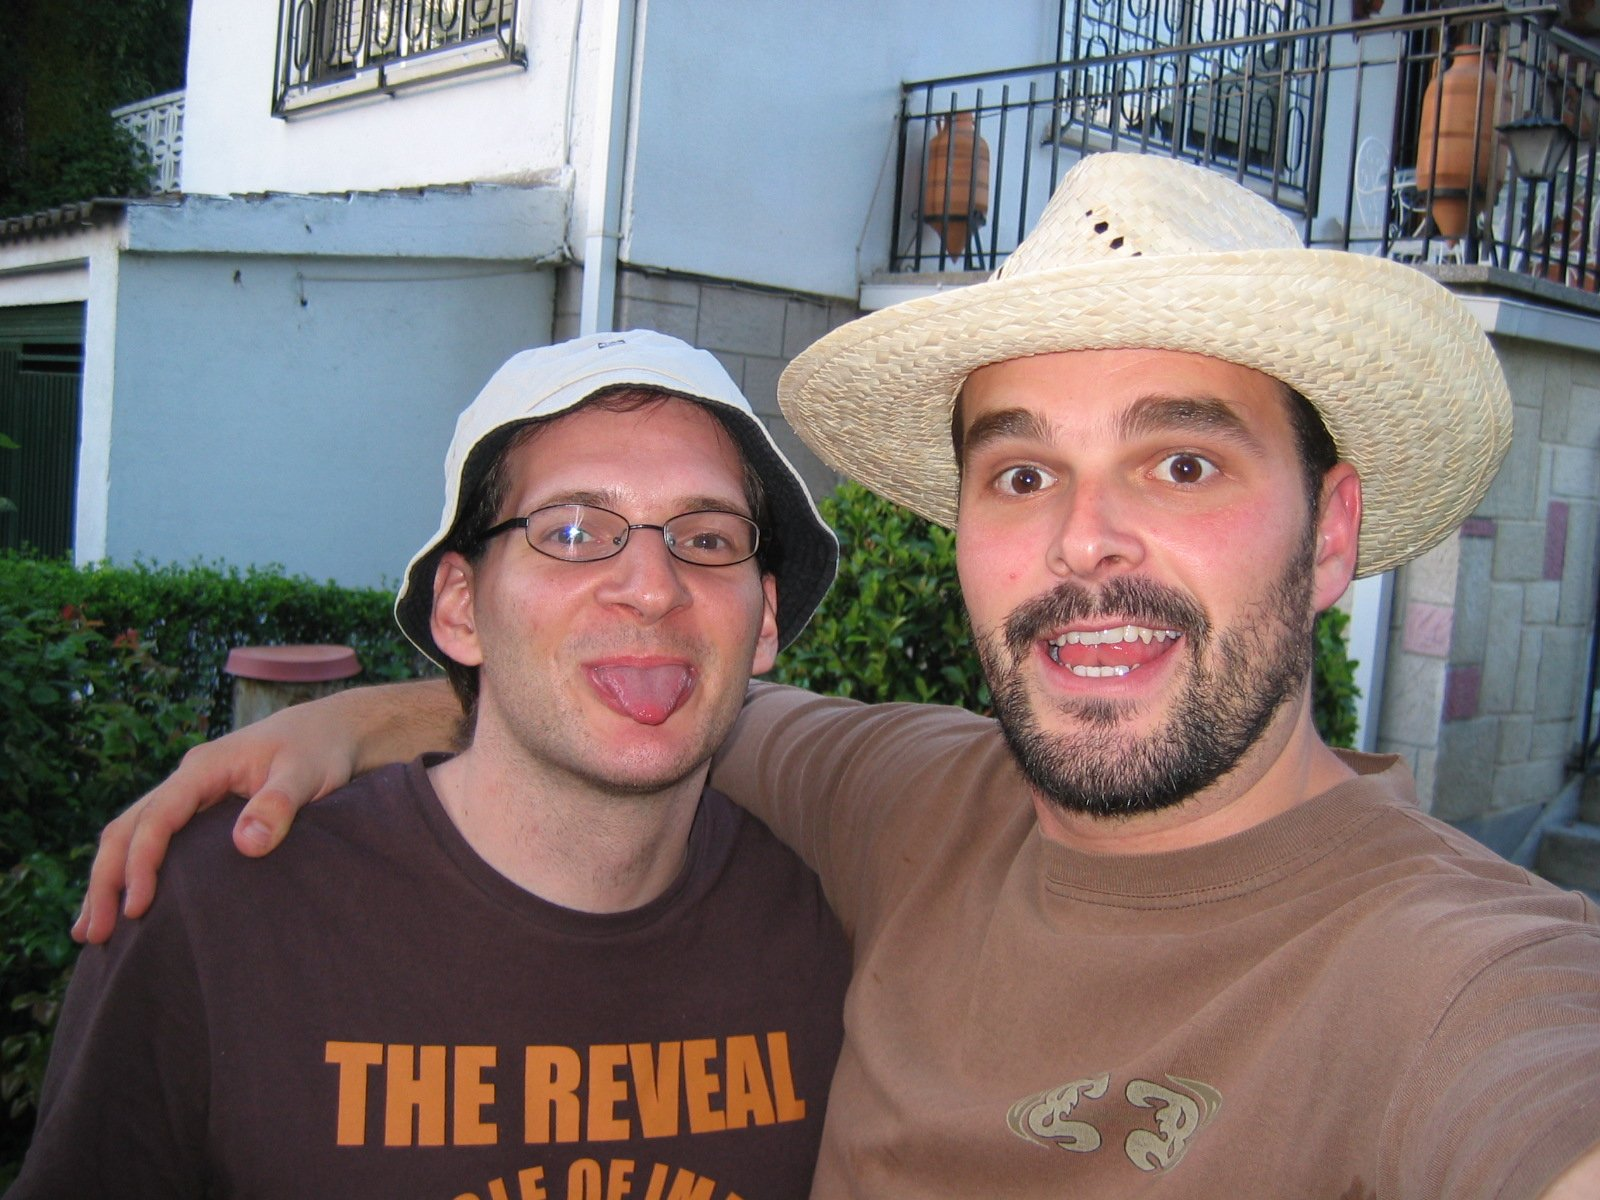
\includegraphics[width=8cm]{figs/martin.jpg}
\end{center}

\end{frame}

\end{document}
